\usetikzlibrary{positioning}

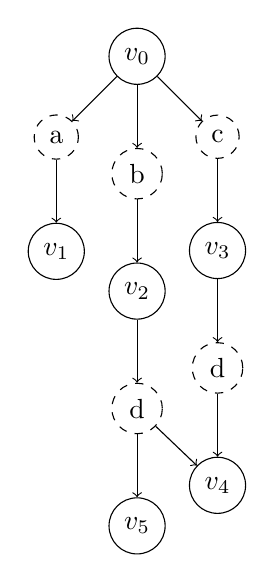
\begin{tikzpicture}[every node/.style={draw,circle},node distance=.8cm]

\node (0) {$v_0$};
\node[dashed,below left = of 0 ] (a) {a};
\node[dashed,below = of 0 ] (b) {b};
\node[dashed,below right = of 0 ] (c) {c};

\node[below = of a ] (1) {$v_1$};
\node[below = of b ] (2) {$v_2$};
\node[below = of c ] (3) {$v_3$};

\node[dashed,below = of 2 ] (d2) {d};
\node[dashed,below = of 3 ] (d3) {d};

\node[below = of d3 ] (4) {$v_4$};
\node[below = of d2 ] (5) {$v_5$};

\path[->,every node/.style={font=\footnotesize,fill=white}]
(0) edge (a)
	edge (b)
	edge (c)
(a) edge (1)
(b) edge (2)
(c) edge (3)
(2) edge (d2)
(3) edge (d3)
(d2) edge (4) edge (5)
(d3) edge (4)
;

\end{tikzpicture}